\apendice{Especificación de diseño}

\section{Introducción}
En este punto vamos a hacer el diseño inicial de las clases de la aplicación y del diseño de paquetes en el que estarán contenidas.

\begin{figure}[h]
	\centering
	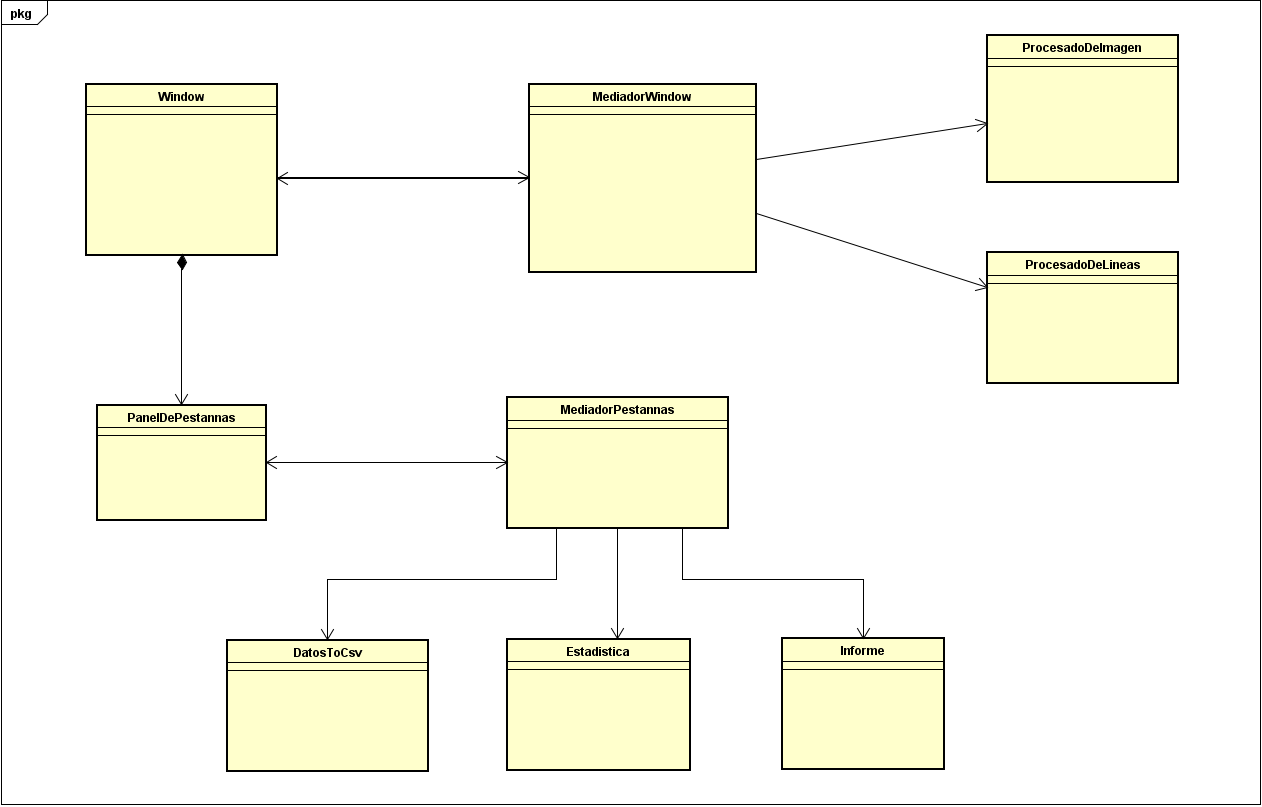
\includegraphics[width=.99\textwidth]{DiaClases}
	\caption{Diagrama de clases inicial}
	\label{fig:C.1.1}
\end{figure}
 


\subsection{Clases}
En esta parte vamos a hacer una breve descripción del contenido de cada clase y su función.

\begin{itemize}
\item Window:
Esta clase contendrá la ventana principal, menús, el panel de pestañas y la imagen sobre la que dibujar.
\item PanelDePestannas:
Esta clase contendrá la botonería y la interacción con la imagen a evaluar.
\item ProcesadoDeImagen:
Esta clase contendrá el tratamiento que tiene que llevar la imagen para la extracción de características a evaluar.
\item ProcesadoDeLineas:
Esta clase contendrá el procesado de las lineas obtenidas por el procesado de la imagen y el resultado final que obtendremos.
\item Informe: 
Esta clase contendrá la generación del informe (Tabla) de estadísticas en formato LaTex para poder exportar fácilmente a un documento PDF.
\item DatosToCsv:
Esta clase contendrá el paso de los datos que contiene la tabla a un documento en formato csv del que desde Excel podemos extraer fácilmente los datos.
\item Estadistica: 
Esta clase contendrá el calculo de los datos estadísticos y la clasificación de las lineas según su orientación.

\end{itemize}

\subsection{Paquetes}
En este punto vamos a hacer una breve descripción de cada paquete y de su contenido dentro de la aplicación.

\begin{itemize}
\item Gui:
Este paquete contendrá todos los elementos gráficos de la aplicación y todos lo que se corresponde con interacción con el usuario.
\item Código: Este paquete contendrá todas las clases de calculo que necesitara la aplicación:
	\begin{itemize}
	\item Estadísticas:
	Este paquete contendrá las clases del calculo de estadísticas.
	\item Informes:
	Este paquete contendrá la generación del informe LaTex
	\item Procesado:
	Este paquete se va a encargar tanto del procesado de la imagen 			como del procesado de los segmentos extraídos hasta conseguir los 		segmentos finales.
	\end{itemize}
\end{itemize}

\begin{figure}[h]
	\centering
	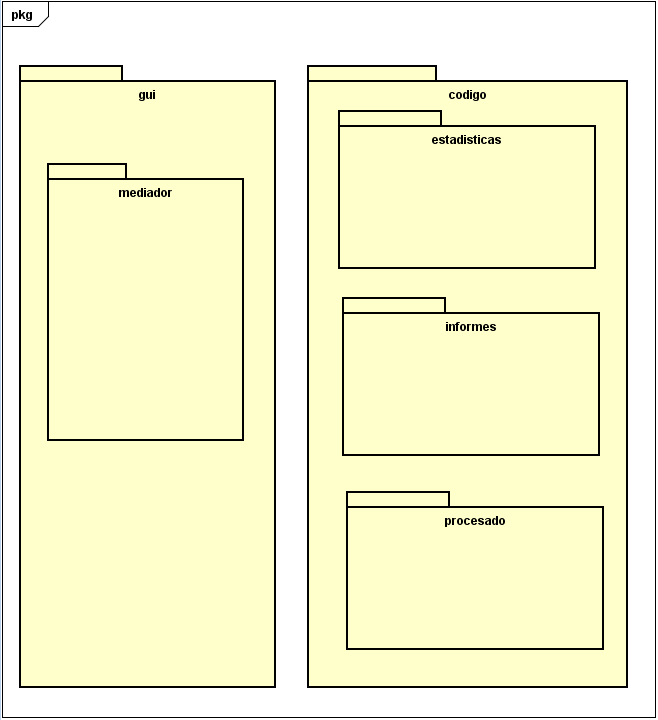
\includegraphics[width=.99\textwidth]{DiaPackages}
	\caption{Diagrama de paquetes inicial}
	\label{fig:C.1.2}
\end{figure}


\section{Diseño de datos}

\section{Diseño procedimental}

\section{Diseño arquitectónico}


